\chapter{Entwicklung der User Experience mit Verwendung des Google Design Sprints}

Die Entwicklung eines nutzerfreundlichen und effektiven UX-Design-Konzepts zur Abstimmung von Schichtwechseln wurde mithilfe des GDS gemacht. Dieser ist ursprünglich für fünf Tage entwickelt worden, um Probleme zu lösen und neue Ideen zu testen. Da der GDS als Einzelperson durchgeführt wurde, wurde er in diesem Projekt zeitlich angepasst.

\section{Phase 1: Verstehen und Definieren}
In der ersten Phase werden die benötigten Informationen gesammelt und analysiert, um das Problem umfassend zu verstehen und klar zu definieren. Die Problemstellung und Zielsetzung wurden bereits in der Einleitung ausführlich behandelt, daher wird in diesem Kapitel direkt auf die praktische Anwendung der nächsten Phasen eingegangen.

\section{Phase 2 und 3: Skizzieren und Auswahl der Idee}
In der Skizzieren Phase beginnt der Prozess der Designerstellung. Hierbei wurden sich zunächst die benötigten Seiten überlegt, um die benötigten Aufgaben und Anforderungen zu erfüllen. Dazu gehört eine Übersichtsseite auf der alle aktuellen Tauschangebote stehen und worüber der Nutzer zu allen weiteren Seiten gelangt, z.B. die zum Hinzufügen und zum Annehmen eines Tauschangebots, sowie eine Seite, auf der der Nutzer seine angenommen Schichten sehen kann und individuelle Einstellungen vornehmen kann. 

Die erste Version der Übersichtsseite war zunächst für einen Desktop ausgelegt (siehe Abbildung \ref{Version1_Desktop}). 

\begin{figure}[h]
    \centering
    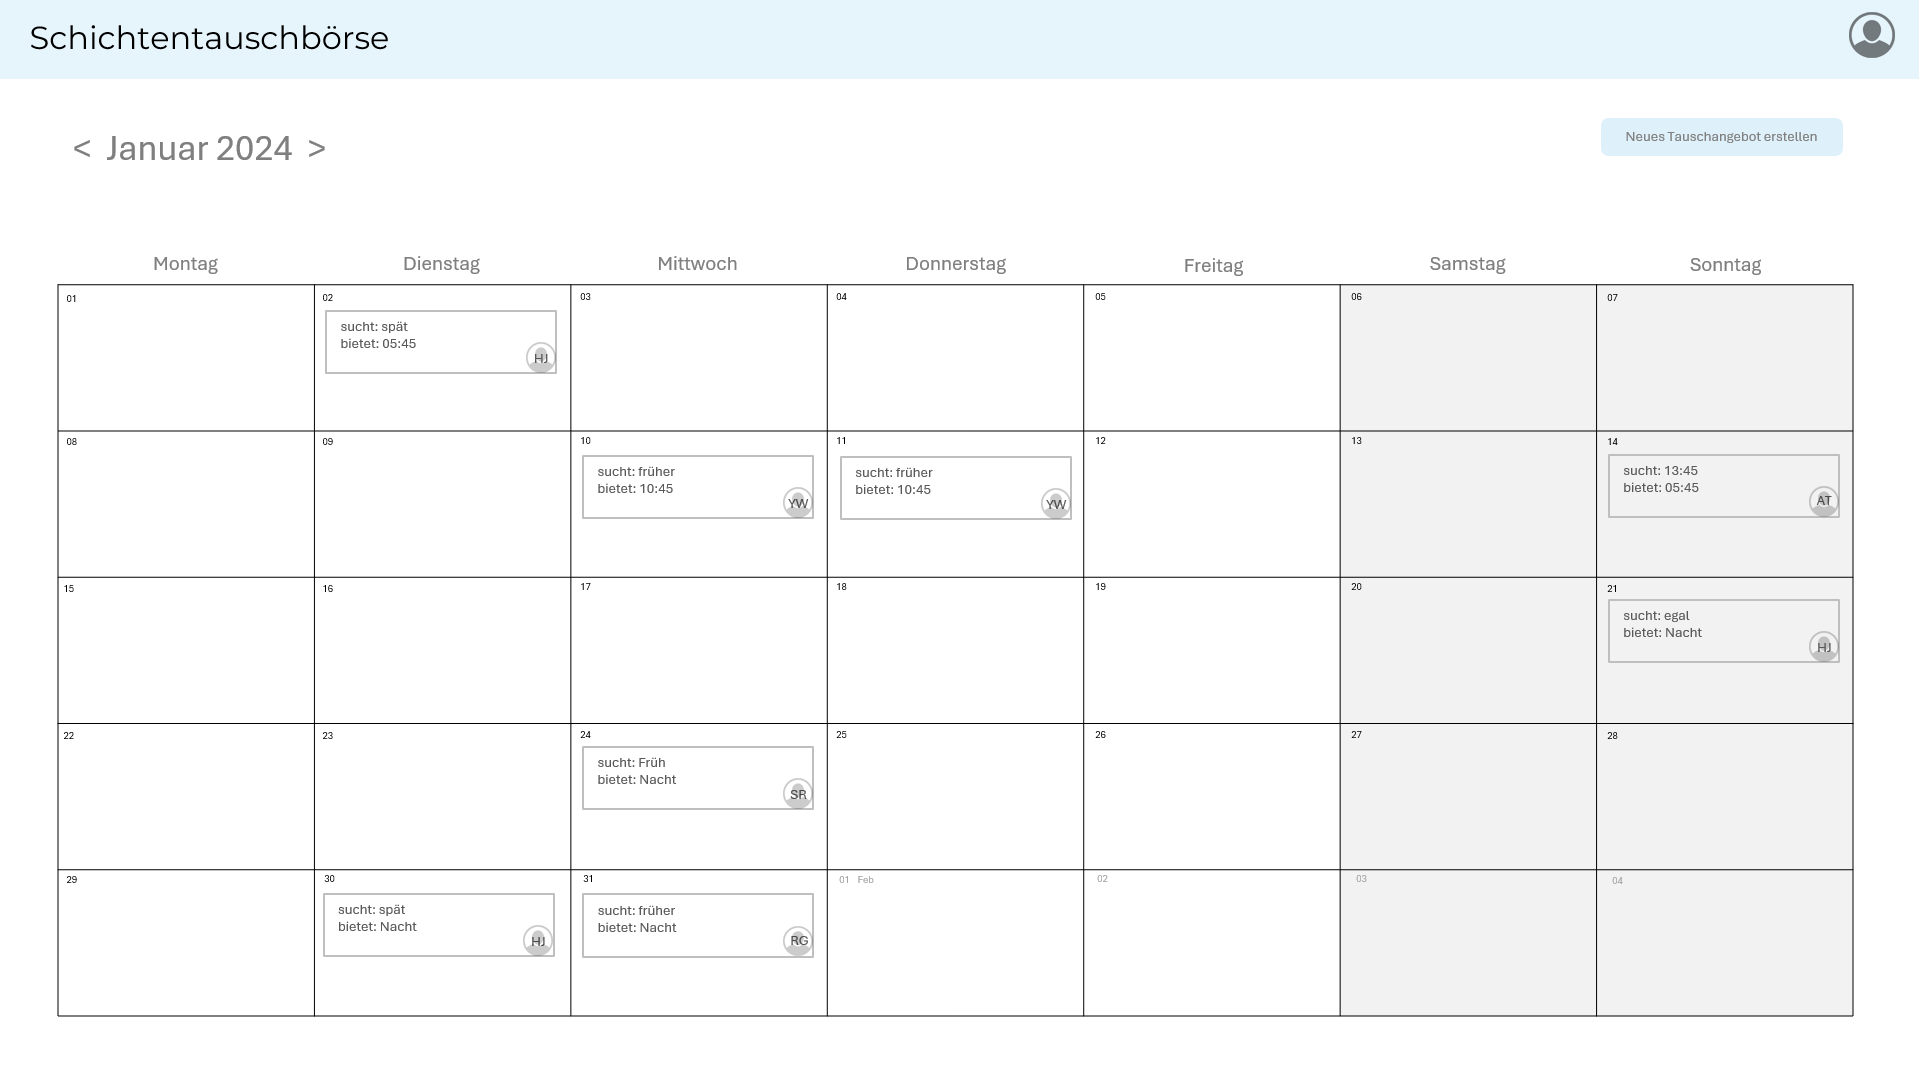
\includegraphics[clip,width=0.9\linewidth]{images/Version1_Desktop.png}
    \caption[Erste Version der Übersichtsseite für den Desktop]{Erste Version der Übersichtsseite für den Desktop}
    \label{Version1_Desktop}
\end{figure}

Über den User auf der rechten Seite im Header kommt der Nutzer zu der Einstellungsseite, über den Namen der Anwendung links im Header wird der Nutzer wieder auf die Übersichtsseite zurückgeleitet. 
Auf dieser ist groß der Kalender des aktuellen Monats zu sehen. 
Links über dem Kalender steht der Monat, welcher aktuell zu sehen ist, über die Buttons daneben kann zum nächsten oder vorherigen Monat gesprungen werden. 
Rechts über dem Kalender ist der Button “Neues Tauschangebot erstellen” platziert, worüber der User eine neue Anfrage zum Schichttausch erstellen kann. 
Direkt über dem Kalender sind die Wochentage ausgeschrieben und das Wochenende im Kalender in einem hellen Grauton hinterlegt, um es leicht von der restlichen Woche abzuheben. 
Im Kalender sind bereits Tauschangebote eingetragen, welche das Schema der Liste aus WhatsApp haben. 
Durch das anklicken dieser, kann der Nutzer die Tauschanfrage annehmen oder das Tauschen wieder abbrechen und zur Übersichtsseite zurückkehren.

Bei der Übertragung des Designs in die Handy-Version wurden einige Schwachstellen identifiziert. Die Darstellung des Desktop-Designs auf dem Handy führt dazu, dass die Schrift aufgrund der kleinen Größe schlecht lesbar war (siehe Abbildung \ref{Version12_Handy}). 

\begin{figure}[h]
    \centering
    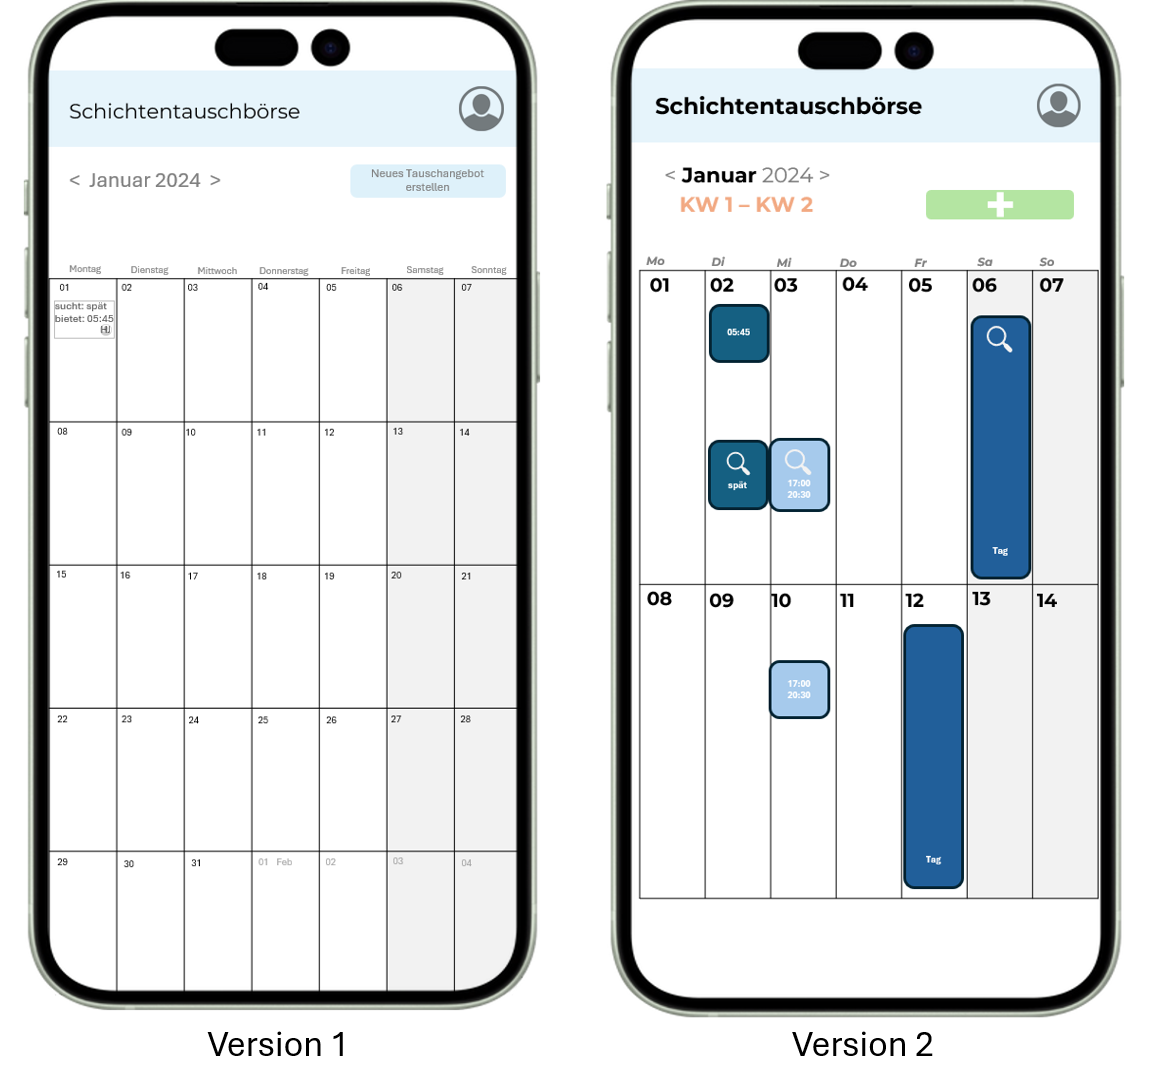
\includegraphics[clip,width=0.75\linewidth]{images/Version12_Handy.png}
    \caption[Erste und zweite Version der Übersichtsseite für das Handy]{Erste und zweite Version der Übersichtsseite für das Handy}
    \label{Version12_Handy}
\end{figure}

Da die meisten Nutzer die App wahrscheinlich auf dem Handy verwenden möchten, wurde das Design in Version 2 entsprechend angepasst.

Um in der Kalenderübersicht die Tauschanfragen gut lesbar und nutzerfreundlich darzustellen, werden statt fünf Wochen nur noch zwei Wochen angezeigt (siehe Version 2 in Abbildung \ref{Version12_Handy}). 
Aufgrund der schmaleren Handybildschirme wird ein Teil der Wörter durch Piktogramme ersetzt, z.B. wurde beim “Neues Tauschangebot erstellen” Button der Text durch ein Plus ersetzt. Dadurch wird Platz gespart und die Funktion wird klarer erkannt. 
Außerdem werden die Wochentage nicht mehr ausgeschrieben. Eine weitere Änderung ist, dass die Schichten in den gesuchten/gebotenen Zeit Blöcken am Tag abgebildet (siehe Version 2 in Abbildung \ref{Version12_Handy}).

Allerdings wurde festgestellt, dass der Kalender unübersichtlich wird, wenn mehrere Tauschangebote an einem Tag sind oder wenn welche zum gleichen Zeitpunkt angefragt werden. 
Deswegen wird eine weitere Version erstellt, in der die Schichten nicht mehr nach dem Zeitpunkt sortiert sind, sondern in einem Block organisiert, was eine bessere Übersicht ermöglicht (siehe Abbildung \ref{Version3_Handy}).

\begin{figure}[h]
    \centering
    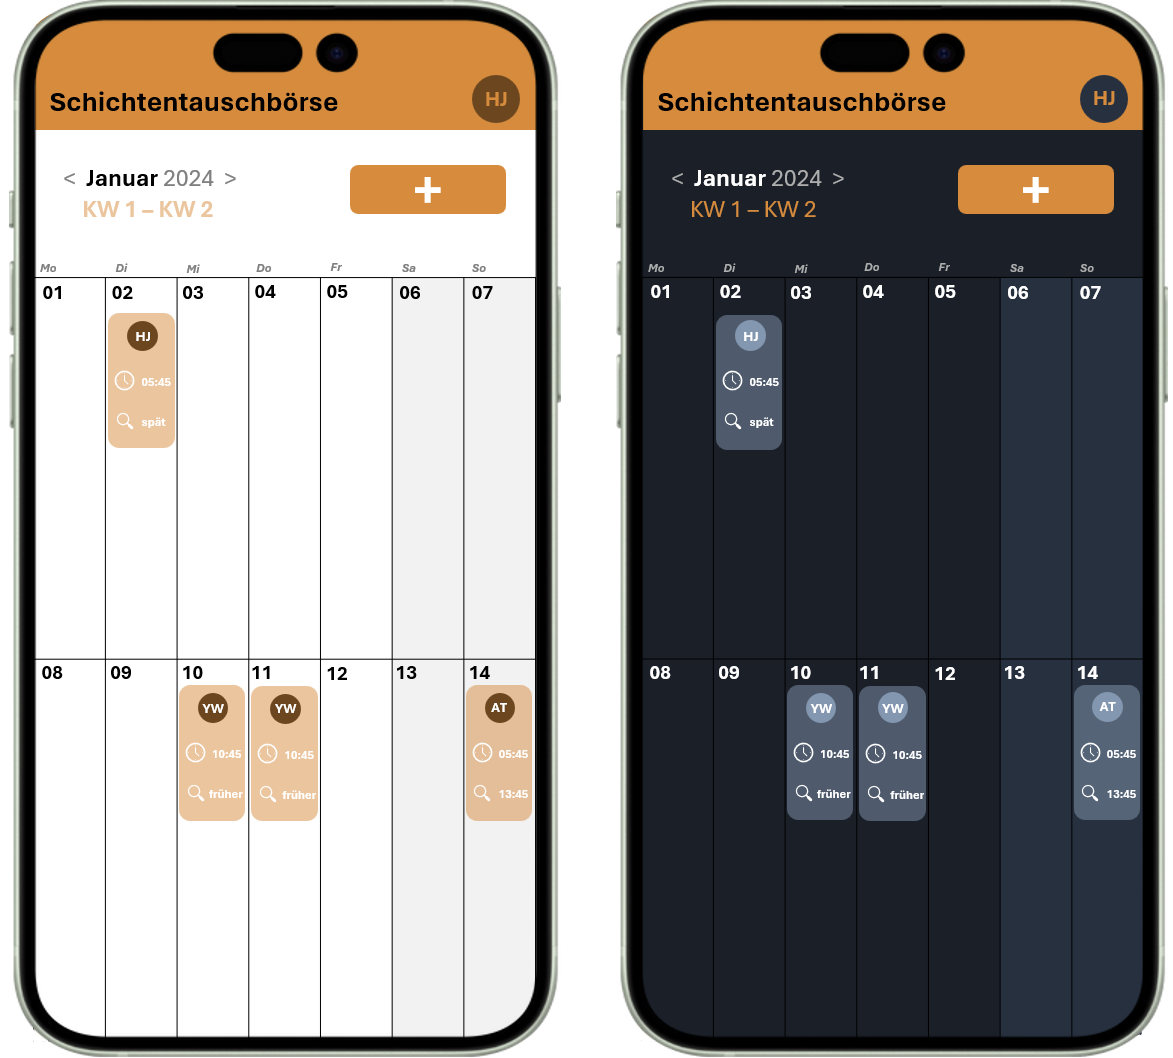
\includegraphics[clip,width=0.75\linewidth]{images/Version3_Handy.png}
    \caption[Dritte Version der Übersichtsseite für das Handy, im Light Mode und Dark Mode]{Dritte Version der Übersichtsseite für das Handy, im Light Mode und Dark Mode}
    \label{Version3_Handy}
\end{figure}

Des weiteren wurde die Hauptfarbe von einem hellen Blau zu einem Orange gewechselt, welches wärmer und aktiver wirkt. Da der Dark Mode in den letzten Jahren stark an Popularität zugenommen hat \cite{diva2020darkmode} wird für die Anwendung auch ein Farbkonzept erstellt (siehe Dark Mode in Abbildung \ref{Version3_Handy}). 

Für die dritte Version wurde sich letztendlich entschieden. Darauf aufbauend wurden die weiteren Seiten der Anwendung im Light Mode gestaltet.

\section{Nutzerumfrage}
